\documentclass[a4paper,12pt,hidelinks]{report}

%%Pacchetti utili anche se non necessari

\usepackage{amsfonts}
\usepackage{amsmath}
\usepackage{latexsym}
\usepackage{tabularx}
\usepackage[italian]{babel}
\usepackage[bookmarks=true]{hyperref}
\usepackage{url}
% \usepackage{subfigure}
\usepackage{epstopdf}
\usepackage[utf8]{inputenc}
% \usepackage[utf8x]{inputenc}
\usepackage{listings}
\usepackage{graphicx}
\usepackage{usecases}
%-------------------------------------------

% \title{Progettazione sito web\\ ''B\&B La Vecchia Posta''}
% \author{Daniele Di Pompeo \\mat. 226766}
% \annoaccademico{2013-2014}
\begin{document}
\begin{titlepage}
  \begin{center}
  % Upper part of the page
    
\includegraphics[width=0.5\textwidth,keepaspectratio=true]{../img/logo}\\[1cm]    
    \textsc{\LARGE Specifiche dei requisiti}\\[0.6cm]
    \textsc{\LARGE  sito: ``B\&B La Vecchia Posta''}\\ [2.0cm]

  % Author and supervisor
    \begin{minipage}{0.8\textwidth}
      \begin{flushleft} \large
	\emph{Autore:} Daniele Di Pompeo \\[0.5cm]
	\emph{Versione documento: 1.0}\\[0.5cm]
	\emph{Data emissione del documento: \today}\\[0.5cm]
      \end{flushleft}
    \end{minipage}
  \end{center}
\end{titlepage}

\tableofcontents

%----------------------------------------------------
\begin{abstract}
  In questo documento verranno descritti nel dettaglio tutti i requisiti funzionali e non funzionali individuati per la realizzazione del sito web del B\&B La Vecchia Posta.
  Per la realizzazione del nuovo sito web sono state utilizzate le informazioni sul traffico dati utilizzando ``Google Analytics''. Sono stati presi in visione i siti web di altre strutture
  locali e nazionali per rendere la versione 2.0 del sito del B\&B La Vecchia Posta utilizzando tutte le nuove tecniche del web 2.0.
  \par Nella prima parte di questo documento si riporta una descrizione dell'attività del committente ponendo l'attenzione sui dati statici raccolti.
  \par Nella seconda parte vengono descritti in maniera puntuale i requisiti funzionali per la realizzazione del nuovo sito web.
  \par Come framework di sviluppo verrà utilizzato ``beContent'' tool sviluppato dall'università dell'Aquila, del quale il sottoscritto è uno sviluppatore.
  \par Nella stesura di questo documento si fa presente al lettore che in alcune sezioni la figura del committente e del progettista vengono specificatamente separate mentre in altre si tende a 
  descriverle come un'unica persona. Questo perchè in alcuni punti del documento è risultato conveniente separare le due figure nell'ipotesi di un cambiamento futuro, nel quale il progettista 
  non è anche il committente.
\end{abstract}

\chapter{Generalità}

\section{Il Committente}
  Il B\&B La Vecchia Posta, inaugurato nell'Agosto del 2010, è situtato in Via Amiternum n.6 nel comune di Cagnano Amiterno, a pochi chilometri dal centro della città di L'Aquila.
  Offre ai suoi clienti 6 spaziose camere tutte con bagno privato, ampio spazio verde di proprietà garantendo ai suoi clienti il massimo confort e relax. 
  Si riporta una veduta aerea dell'area del B\&B per far rendere conto al lettore la posizione geografica e la conformazione dello spazio (fig.\ref{fig:bbArea}). 

  \begin{figure}[h!]%
    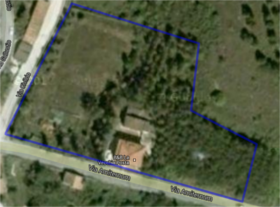
\includegraphics[width=0.6\textwidth,keepaspectratio=true]{../img/bbArea1}
    \centering
    \caption{veduta area del B\&B La Vecchia Posta}%
    \label{fig:bbArea}%
  \end{figure}
  Il B\&B è a conduzione familiare, il titolare, l'autore di questo documento, è coadiuvato dai genitori Emanuela e Nando che hanno avuto ed hanno un ruolo importante 
  nell'esercizio dell'azienda.

\section{Situazione attuale}
  Il B\&B La Vecchia Posta risulta essere titolare di un dominio web dall'url \url{www.vecchiaposta.it}, al momento non sono stati previsti alias. 
  \par Il sito web è stato realizzato nel 2010 dalla \textit{Fermenti Grafici}, web agency aquilana, che a titolo di amicizia si è occupata della realizzazione
  del comparto grafico (logo, foto, template) ed ha, inoltre, fornito gratuitamente l'hosting.
  \par Per lo sviluppo della prima versione del sito web del B\&B è stato utilizzato WordPress, uno dei più famosi CMS nel mondo del web e ampliato con l'installazione 
  di plug-in (google sitemap, contact form 7, ecc)  per fornire al sito alcune funzionalità di cui il committente aveva bisogno.
  \par Ad oggi il sito web risulta essere completamente gestito dal sottoscritto ed è hostato dalla web farm ARUBA.
  \\Dall'analisi dei dati raccolti il sottoscritto si è reso conto che molta della pubblicità programmata su internet, tramite il servizio \textit{Google Adword}, 
  non portava ai risultati attesi, quindi è sorta la neccessità di aggiornare il sito web attuale.
  Si mostra lo screenshot della home page attuale
  \begin{figure}[h!]%
    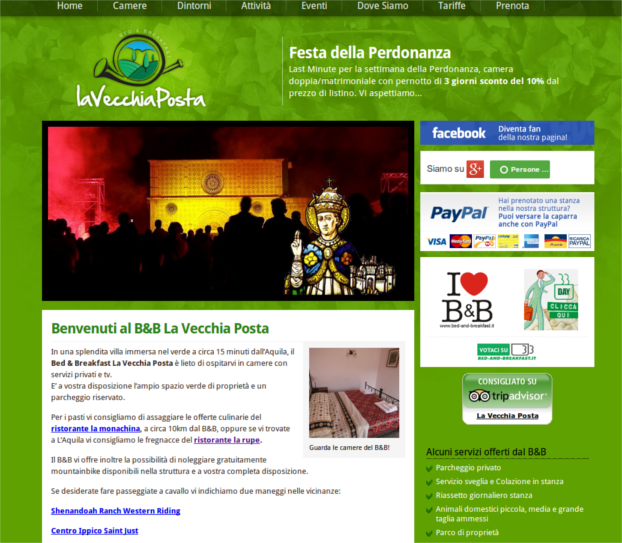
\includegraphics[width=0.95\textwidth,keepaspectratio=true]{../img/homepage}
    \centering
    \caption{Home page}%
    \label{fig:googleHomePage}%
  \end{figure}
  
\subsection{Aspetti rilevanti del sito}
  Da interviste effettuate sui clienti del B\&B risulta essere di gradevole impatto il sito, grazie ad una grafica curata minuziosamente.
  Inoltre gli utenti apprezzano la navigazione del sito grazie alla facile barra di navigazione primaria e secondaria, ove presente, risulta essere sopra la media ma non 
  senza problematiche, analizzate alla sezione \ref{subsec:difetti}.

\subsection{Principali pregi}
  L'intero sito web non ha oggetti in flash, quindi completamente navigabile da dispositivi mobile, anche se non ha una versione responsive.
  \\La risoluzione base è 1024px, al momento della realizzazione era la risoluzione più utilizzata, sono stati evitati scroll orizzontali. 
  \par La home page effettua 79 HTTP Request per un peso complessivo di circa 771Kb scaricabili in circa 20 secondi con una connessione a banda larga di velocità media (4Mb).
  \par La struttura dell'intero sito è sempre coerente fornendo uno spazio per l'immagine principale della pagina, che può anche essere uno slider 
  e dello spazio binanco per il testo, rendendo la lettura gradevole non affaticando gli occhi del lettore grazie anche all'utilizzo di un font sans-serif.

\subsection{Principali difetti} 
\label{subsec:difetti}
  Non è prevista una versione mobile del sito, che lo rende di dificile utilizzo tramite device mobile (tablet, smartphone, padfone).
  \par I principali difetti sono legati dalla difficoltà nel raggiungere il collegamento per effettuare una richiesta di prenotazione, accessibile 
  solamente tramite la barra di navigazione o tramite il link nascosto dietro il testo dell'offerta attiva.
  \\ Questo è confermato, anche dai dati statistici raccolti da Google Analytics, che mostrano come l'utente navighi nel sito per poco meno di 2 minuti e 
  lo abbandoni prima di inviare una richiesta di prenotazione. Ciò è evidenziato dal fatto che il link \textit{prenota} non risulta mai essere cliccato.
  \begin{figure}[h!]%
    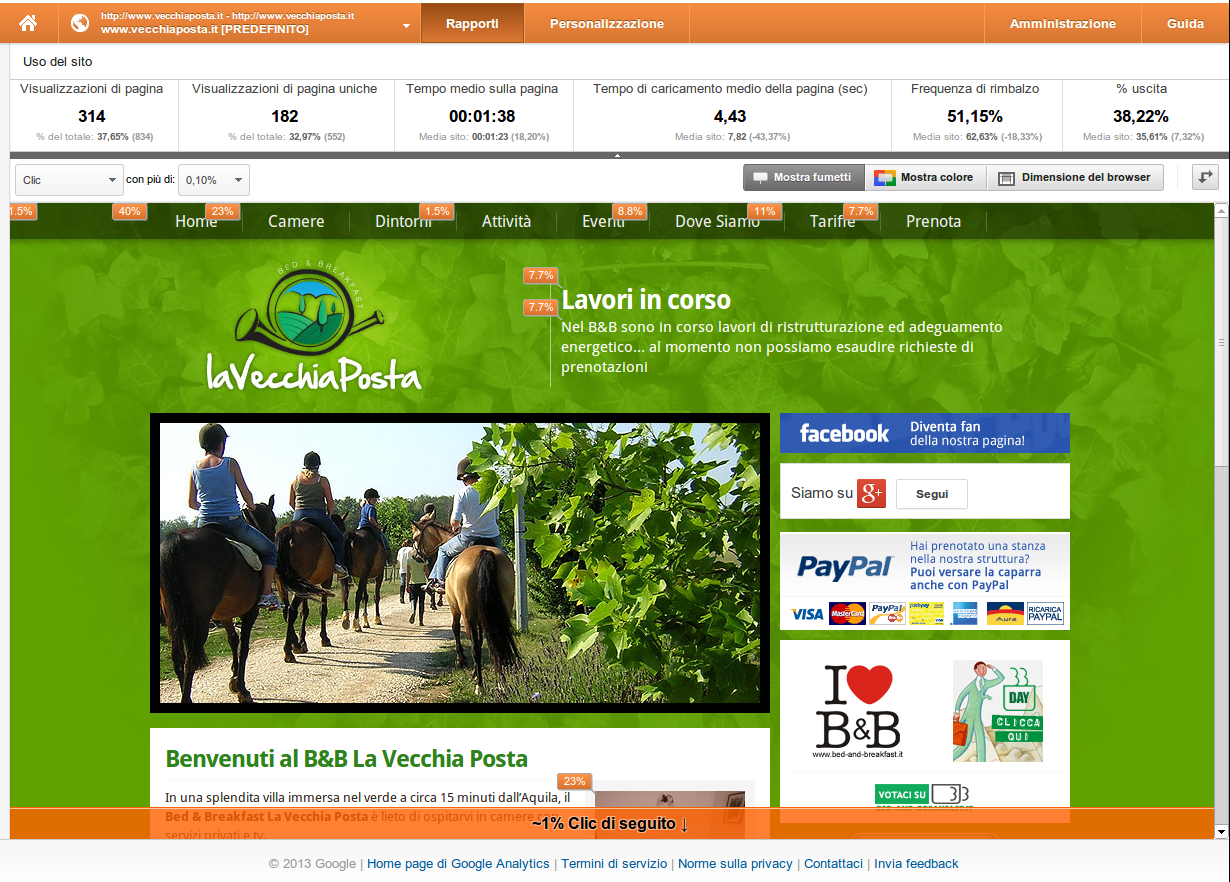
\includegraphics[width=0.95\textwidth,keepaspectratio=true]{../img/googleAnalyticsDoc1}
    \centering
    \caption{Dati statistici navigazione home page}%
    \label{fig:googleHomePage}%
  \end{figure}
  \par Dall'immagine fig.\ref{fig:googleHomePage} risulta evidente che la barra di navigazione posta sopra il logo rende difficoltoso all'utente medio comprendere 
  quale sia il vero link alla home page. Si notano alcuni click sullo spazio negativo della barra di navigazione a sinistra della label \textit{Home}
  (più del 40\% degli utenti).
  \par Nella sezione \ref{sec:appendice1} vengono riportare altre immagini e dettagli a supporto degli aspetti negativi della versione attuale 
  del sito web in base ai dati statici raccolti.
  \par Inoltre si riscontra che non è prevista la modifica della grandezza del font, non permettendo una facile navigazione a persone ipovedenti. 
  Analizzando il tema del sito con il serivizio offerto dal sito \url{http://colorfilter.wickline.org/} risulta perdere completamente l'effetto desiderato mostrandosi piatto 
  e privo di effetti grafici, almeno per le forme di daltonismo più comuni.

\section{Obiettivi generali del nuovo sito}
  La nuova versione del sito web dovrà eliminare queste problematiche, invogliando gli utenti ad inviare più richieste di prenotazioni
  inserendo nella parte ``sopra la piega'' una scorciatoia al ``form'' di prenotazione.
  \par Il nuovo sito inoltre, nella versione base dovrà fornire le informazioni ad oggi presenti migliorando la navigabilità spostando la barra di navigazione 
  al di sotto del logo del B\&B, aspetto grafico maggiormente utilizzato.
  \par L'home page del sito dovrà restare leggera e non dovrà prevedere nessuna funzionalità in flash, che la renderebbe inaccessibile dai dispositivi mobile.
  L'intento è di fornire ``\textit{sopra la piega}`` tutte le informazioni utili come:
  \begin{itemize}
    \item collegamento all'home page al click sul logo
    \item barra di navigazione al di sotto del logo
    \item slider di immagini
    \item form per la richiesta di disponibilità
    \item preview dell'offerta attiva
  \end{itemize}
  Si è scelto quindi di utilizzare il servizio di vendita di temi di \url{www.themeforest.com} acquistando un tema grafico che risponda alle nostre esigenze.
  \par La nuova versione del sito dovrà essere ''responsive'' garantendo la completa compatibilità con i maggiori device che ad oggi accedono ad internet.
  \\In particolare:
  \begin{itemize}
    \item 1200px Desktop
    \item 1024px iPad landscape and netbook
    \item 768px 7inch tablet
    \item 368px mobile phone
  \end{itemize}
  Prendendo come risoluzione base 1200px essendo circa il 90\% degli utenti ad utilizzarla \footnote{Fonte \url{http://www.w3schools.com/browsers/browsers_display.asp}}
  ed inoltre facendo attenzione alla compatibilità fra i differenti browser (chrome, firefox, safari, explorer ed opera).

\section{Utenti}
  Dall'analisi effettuata risultano essere stati individuati tre categorie di utenti:
  \begin{itemize}
    \item L'Amministratore
    \item L'utente occasionale (utente che raggiunge il sitoweb involontariamente) (aka \textit{Utente})
    \item Il Cliente, navigatore di internet che effettua una richiesta di prenotazione e/o è stato già cliente dell'azienda.
  \end{itemize}
  \begin{center}
    \begin{tabular}{||m{3cm}||m{4cm}|m{1,5cm}||m{4cm}|m{1,5cm}||}
      \hline
	\textbf{Categoria di utenti} & \textbf{Bisogni principali degli utenti in relazione al sito} & Priorità & \textbf{Obiettivi del committente} & Priorità \\
      \hline
	Amministratore & mantenere aggiornarnate le informazioni presenti sul sito & alta 
	& fornire all'amministratore le informazioni aggiornate da inserire nel sito web & alta\\
      \hline
	Utente & reperire le informazioni di contatto, prendere visione della struttura & alta, media
	      & impressionare l'utente casuale invogliandolo ad effettuare una prenotazione,  & alta\\
      \hline  
	Cliente & reperire informazioni di contatto, visionare il tariffario, effettuare una richiesta di prenotazione & alta, media, alta & mantere ottimi rapporti con
	il cliente abitudinario, invogliare il ``passaparola'' dei clienti & alta, alta\\
      \hline
    \end{tabular}
  \end{center}
  \subsection{Profilo degli utenti}
    \begin{itemize}
    \item \textbf{Cliente}: sono i navigatori di internet che cercando una destinazione per le proprie vacanze si sono imbattuti sul sito web della struttura 
    e hanno la volotà di inviare una richiesta di disponibilità. 
    Rientrano in questa categoria di utenza anche i clienti ``storici'' del B\&B avendo già soggiornato nella struttura in un'altra occasione.
    \item \textbf{Utente}: sono i navigatori di internet definiti come i visitatori di rimbalzo, ovvero quegli utenti che non volendo sono giunti sul sito 
    internet del B\&B \footnote{Sono questi utenti a fornire feedback sulla scelta di inserire una scorciatoia al form per le prenotazioni}.
    \end{itemize}

\section{Scenari d'uso}
  \par
  \begin{itemize}
  \item \textbf{Cliente}: Michela, signora sulla cinquantina residente in lombardia, lavora presso un'agenzia per il turismo.
  \\La sua passione, forse anche legata al suo lavoro, la spinge sempre a scoprire nuovi luoghi e nuove bellezze naturalistiche, magari trovando anche 
  nuovi clienti per il suo impiego.
  \\ Decide di prenotare una vacanza di qualche giorno in Abruzzo, precisamente nel Parco Nazionale del Gran Sasso e monti della Laga. 
  Navigando in internet e utilizzando i portali più famosi del settore \footnote{\url{http://www.bed-and-breakfast.it/}, il più famoso in Italia}.
  Tra i vari B\&B presenti nel portale decide di visionare il sito web dell'azienda.
  Grazie ad una grafica curata decide di effettuare una richiesta di prenotazione. Da allora Michela trascorre le sue vacanze estive nel 
  B\&B La Vecchia Posta.
  
  \item \textbf{Utente}: Antonietta ragazza di 23 anni studentessa di filosofia a Bologna, non è la classica ragazza che gli amici eticheterebbero come ``tecnologica''. 
  Infatti ama utilizzare il suo vecchio telefono nokia con il tastierino numerico e schermo non touch. 
  \par Navigando in internet per una ricerca universitaria inizia a seguire una serie di link pubblicitari per prenotare le sue vacanze a prezzi super stracciati. 
  \\ Non essendo un'abile navigatrice di internet non si rende subito conto di ciò che sta facendo e cliccando su un link piuttosto che su un altro
  arriva sul sito web dell'azienda.
  \\La sua attenzione viene catturata dalle immagini presenti, invogliata ed incuriosita di vedere la natura Abruzzese decide di prenotare una camera.
  Preferendo il contatto telefonico recupera facilmente i recapiti dell'azienda ed effettua una chiamata e prenota la sua vacanza.
  \end{itemize}

\section{Posizionamento competitivo}
  \par Per il nuovo sito si intende migliorare l'indicizzazione sui principali motori di ricerca (google, bing, yahoo) posizionandolo nei primissimi posti 
  seguendo le direttive imposte dai motori di ricerca.
  \\Per ottenere un risutlato di pregio sono stati analizzati siti web di altre strutture locali e nazionali (nelle principali località turistiche)
  per catturare quelle funzionalità che, in prima analisi, potevano sfuggire ma che risultano essere utili.
  \par I siti web locali analizzati sono stati:
  \begin{itemize}
    \item B\&B Camaga
    \item La compagnia del viaggiatore
  \end{itemize}
  mentre per i siti extra-regione sono stati analizzati:
  \begin{itemize}
    \item Il giglio binaco (Sorrento)
  \end{itemize}
  Per l'analisi dettagliata sui siti web analizzati si rimanda alla sezione \ref{sec:appendice2}.

\chapter{Requisiti del sito}

\section{Requisiti di architettura}
  \subsection{Architettura informativa}
   \begin{itemize}
    \item Home
      \begin{itemize}
	\item Camere
	  \begin{itemize}
	    \item Singola
	    \item Doppia
	    \item Tripla
	    \item Quadrupla
	  \end{itemize}
	\item Eventi
	  \begin{itemize}
	    \item Perdonanza Celistiniana
	    \item Festa del Cioccolato
	    \item Sagre e Feste
	  \end{itemize}
	\item Attività
	  \begin{itemize}
	    \item Ippovia del Gran Sassi
	    \item L'anello del Lago di Campotosto
	    \item Da Cagnano al Gran Sasso
	  \end{itemize}
	\item Dintorni
	  \begin{itemize}
	    \item L'Aquila
	    \item Amatrice
	    \item Parco Nazionale del Gran Sasso
	    \item Lago di Campotosto
	    \item Campo Imperatore
	    \item Campo Felice
	  \end{itemize}
	\item Dove Siamo
      \end{itemize}
    \end{itemize}

  \subsection{Navigazione}
    Per quanto riguarda la navigazione del sito sarà necessario organizzare una barra di navigazione orizzontale che permetta all'utente di spostarsi 
    facilmente da una sezione di primo livello ad un'altra. La barra di navigazione di primo livello si è deciso di posizionarla al di sotto del header, 
    che contiene il logo dell'azienda e la preview dell'offerta attiva. 
    \\ Al di sopra del logo si pensa di inserire i collegamenti alle pagine social, link che vengono utilizzati in minor modo.
    Inoltre sempre nella parte alta della pagina viene utilizzato il classico ``marker'' delle mappe come scorciatoia per mostrare velocemente la mappa, 
    una scorciatoia per effettuare una richiesta di prenotazione e i bottoni per la gestione della grandezza dei font.
    \par Per le sezioni di secondo livello si pensa di utilizzare una barra di navigazione verticale per permettere all'utente di spostarsi agevolmente
    nelle varie sezioni interne. Il menu di secondo livello verrà posizionato nella sidebar di destra, appena sotto lo slider, 
    suddividendo lo spazio della pagina in un 70\% destinato ai contenuti ed un 30\% destinato al menu di secondo livello.
    \par Si riporta uno schema della gabbia logica per l'home page del sito. Le altre pagine manterranno una struttura simile all'home page garantendo alta la coesione
    tra i contenuti.
    \begin{figure}[h!]%
      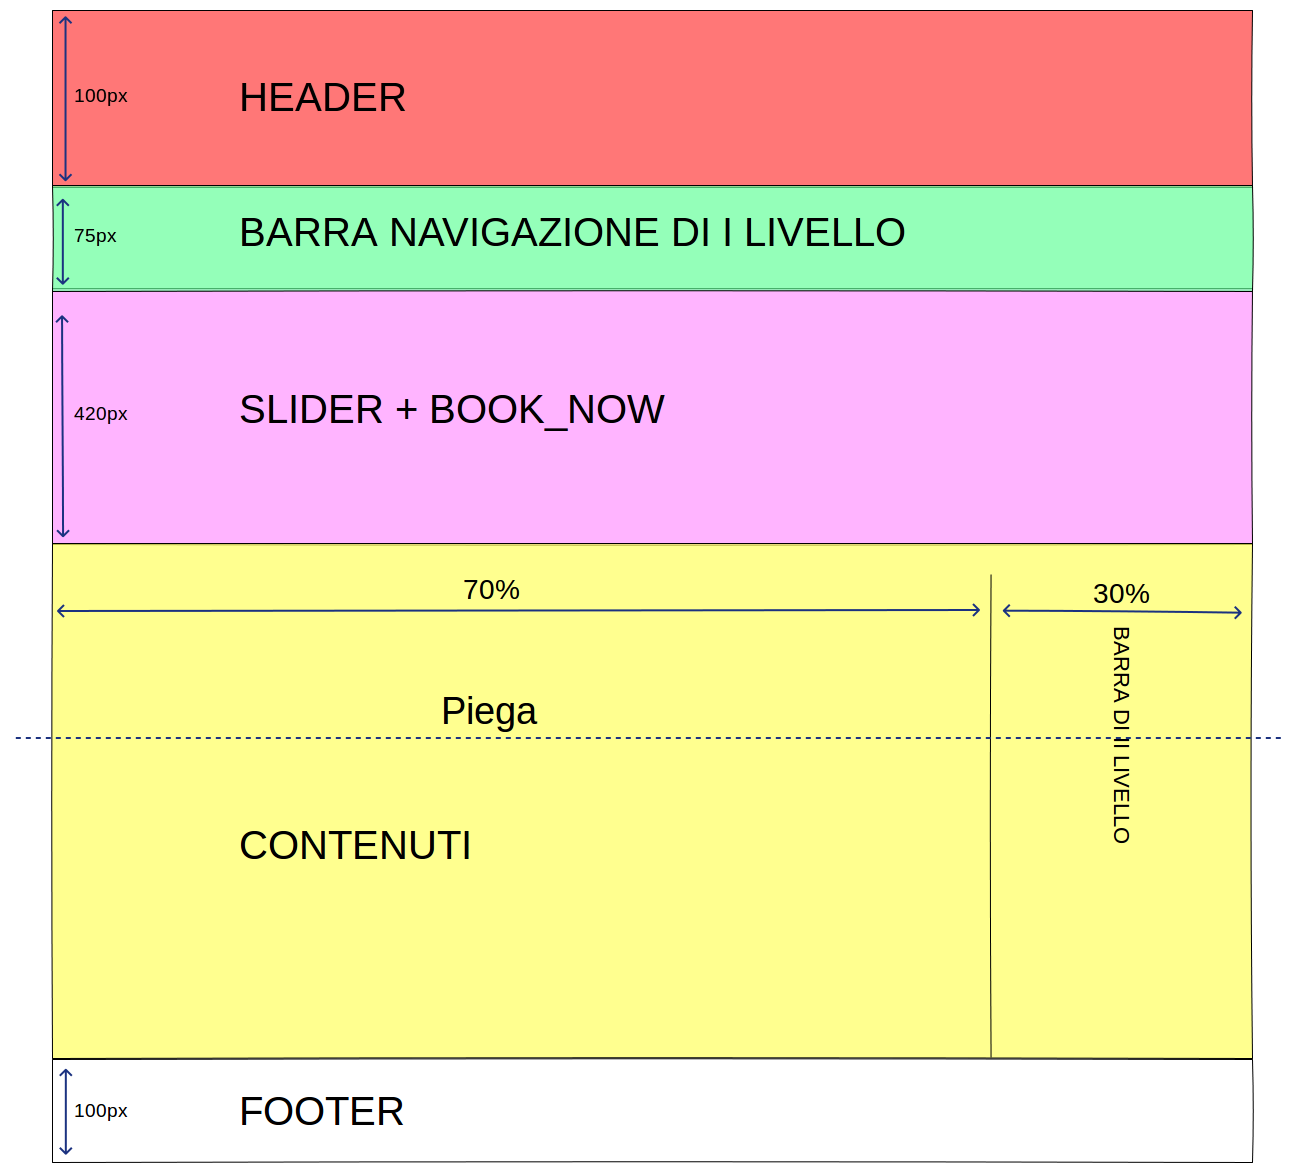
\includegraphics[width=0.95\textwidth,keepaspectratio=true]{../img/gabbiaLogica}
      \centering
      \caption{Gabbia logica}%
      \label{fig:gabbiaLogica}%
    \end{figure}
  \newpage
  
\section{Requisiti di comunicazione}
  \subsection{Identità di marca, tono e stile della comunicazione}
    Semplicità, eleganza e calore sono le caratteristiche che il comparto grafico del sito dovrà rispettare essendo le caratteristiche dell'azienda. 
    Si è scelto una palette di colori che richiami il logo ed i colori della terra, ponendo il focus sulle caratteristiche principali dell'azienda. 
    I colori dominanti per il sito sono il verde e il marrone. 
    \\Nella parte sopra la piega oltre alla scorciatoia al form per la richiesta di disponibilità si è deciso di insere uno slider in modo da ottenere una home page
    stile vetrina, metodo che attualmente è più in voga nei siti internet nel campo del turismo. 
    Nella sezione sotto la piega sono stati collocati invece i contenuti multimediali che risultano essere di minore rilevanza al fine di ottenere una richiesta
    di prenotazione.

  \subsection{Grafica e multimedialità}
    Per il comparto grafico si è pensato di prendere come risoluizione base i 1200px di larghezza, essendo la risoluizione 
    di maggiore utilizzo\footnote{Dati di \url{www.w3schools.com}}.
    Non sono quindi previsti scroll orizzontali ma solo verticali, mantenendo \textit{sopra la piega} tutte le informazioni principali e la barra di navigazione primaria.
    Per mantenere il sito al passo con i tempi si è deciso di renderlo anche responsive, prevedendone una versione per smartphone e tablet oltre che per desktop.
  
  \subsection{Lingua e localizzazione}
    Per lo sviluppo del nuova versione del sito, si è scelto di utilizzare il framework beContent, ciò ci permette in automatico la scelta della lingua preferita dall'utente,
    potendo eliminare i pulsanti sul controllo della lingua. 

\section{Requisiti funzionali}
  \subsection{Casi d'uso}
    Per la realizzazione del nuovo sito internet sono stati individuati, in prima analisi, i seguenti casi d'uso per i singoli attori. 
    \begin{itemize}
    \item Amministratore:
      \begin{enumerate}
	\item UC1: Inserire contenuti
	\item UC2: Aggiornare il sistema
	\item UC3: Mantenere frunzionante il sistema
      \end{enumerate}
    \item Utente: 
      \begin{enumerate}
	\item UC4: Visualizzare le informazioni di contatto
      \end{enumerate}
    \item Cliente: 
      \begin{enumerate}
	\item UC5: Effettuare una richiesta di prenotazione
      \end{enumerate}
    \end{itemize}
    Si rimanda il lettore alla sezione \ref{sec:appendice3} per la lettura dei casi d'uso in forma dettagliata.

  \subsection{Base di dati}
    La nuova versione del sito internet, non utilizzerà la vecchia base dati, ma sarà sviluppata una nuova base di dati rispettando le esigenze 
    del nuovo framework di sviluppo.
    \par Nella nuova base di dati verranno memorizzati tutte le informazioni necessarie al funzionamento di beContent, come la password di amministratore 
    e di tutti gli utenti che devono interagire con lo stesso (attualmente l'amministratore di sistema è anche il committente quindi un solo utente avrà 
    i diritti per l'accesso nell'area di backend del framework).
    Verranno inoltre memorizzati i contenuti delle pagine interne (testo, link, file multimediali).

  \subsection{Sicurezza e privacy}
    Nella versione 1.0 del nuovo sito non è previsto il mantenimento delle informazioni dei clienti su database, ma solamente l'invio tramite email dei dati necessari
    alla prenotazione di una camera.
    All'utente sarà comuque richiesto esplicitamente di accettare le codizioni sull'utilizzo dei propri dati in conformità con la normativa art. 13 del d.lgs. 196/2003.

\section{Requisiti di contenuto}
  Essendo l'amministratore l'unica figura responsabile ad utilizzare il framework, sarà suo compito inserire, modificare ed eliminare i contenuti multimediali del sito.
  \par Le sezioni in lingua straniera (inglese, spagnolo) saranno redatte dal sottoscritto coadiuvato da Antonietta, laureata in lingue straniere (inglese e spagnolo).
  \\Le due lingue straniere scelte sono dovute dal fatto che molte delle visite al sito internet provengono oltre che dall'Italia, dagli Stati Uniti dall'Inghilterra 
  e dal Brasile come viene mostrato dalla figura \ref{fig:googleAnalyticsPaesi} nella sezione \ref{sec:appendice1}''.
  \par La home page dovrà contenere principalmente immagini e poco testo sfruttando immagini d'effetto si riuscirà a catturare l'attenzione dell'utente più facilmente.
  \\Si presume che i contenuti delle sezioni ``Eventi'' e ``Dintorni'' dovranno contenere del testo descrittivo delle foto illustrative per descrivere al lettore in 
  modo chiaro le caratteristiche delle varie sezioni.
  \\ Nelle sezioni ``Camere'' invece si utilizzerà in maniera combinata test ed immagini per descrivere la struttura dell'azienda e una tabulazione per sintetizzare
  le tariffe. Utilizzare la tabulazione rende più leggibile i costi delle varie camere. 
  

\newpage

\section{Requisiti di gestione}

  \subsection{Infrastruttura per l'esercizio del sito}
    Si presuppone di hostare il nuovo sito internet su una web farm che offra anche servizio SMTP per l'invio di email. 
    Il B\&B La Vecchia Posta risulta essere titolare di un dominio internet \url{www.vecchiaposta.it}, non si ha la necessità di registrare alias e altri domini, 
    almeno per il momento.
    \par L'azienda ha inoltre una casella di posta elettronica, \url{info@vecchiaposta.it} utilizzata per la ricezione delle richieste di prenotazioni e per 
    l'invio delle risposte ai clienti. 
    Risulta utile utilizzare i servizi di Antivirus, AntiSpamm che la web farm offre per rendere più confortevole l'utilizzo della mail, eliminando i 
    messaggi indesiderati.
    
  \subsection{Gestione dei sistemi}
    Il sitema sarà affidato in outsourcing, ed è stato scelto come gestore esterno la compagnia Aruba, tra le web farm più in voga al momento.
    \par Nella fase iniziale non è venuta alla luce l'esigenza di richiedere al gestore caratteristiche particolari del server, l'unica esigenza 
    è stata avere la piattaforma su OS Linux, con tecnologia LAMPP.
    Il progettista avrà l'onere di assolvere tutte le beghe burocratiche con la web farm.
    
  \subsection{Gestione del sito}
    Sarà compito del sottoscritto risolvere eventuali bug e di apportare modifiche successive alla pubblicazione della nuova versione. Inoltre il sottoscritto ricoprirà
    la figura del webmaster.
    
  \subsection{Gestione dei contenuti}
    I contenuti multimediali saranno inseriti sempre dal sottoscritto, essendo l'unica figura con i diritti per utilizzare il framework.
    Si riporta una tabella riassuntiva:
    \begin{center}
      \begin{tabular}{||m{6cm}|m{3cm}|m{3cm}||}
	\hline
	  \textbf{Contenuti} & \textbf{Chi li aggiorna} & \textbf{Chi ne autorizza la pubblicazione}\\
	\hline
	  Framework ed i suoi plugin & Amministratore & Amministratore\\
	\hline
	  Immagini e contenuti multimediali & Amministratore & Titolare\\
	\hline  
	  Offerte e News & Amministratore & Titolare \\
	\hline
      \end{tabular}
    \end{center}
    \par Si fa presente che anche se la figura dell'amministratore e del titolare in questo caso risultano le stesse ma si è preferito differenziare i compiti nell'ipotesi
    che, in una fase successiva, le due figure siano ricoperte da persone differenti.
  
  \subsection{Getione degli utenti}
    Gli utenti comunicheranno con l'azienda tramite posta elettronica, inviando un messaggio direttamente o utilizzando l'apposito form presente in tutte le pagine del sito.
    \par Non sono previsti tempi massimi di attesa per le risposte da parte dell'azienda e sarà compito del titolare gestire le comunicazioni con i clienti.

\section{Requisiti di accessibilità}
  \subsection{Prestazioni}
    Non risultano esserci notevoli vincoli prestazionali, si presume di avere un caricamento dell'home page stimato in 1-2 secondi non imponendo un numero 
    massimo di richieste HTTP.
    Inoltre di presuppone di utilizzare più chiamate asicrone con il server per ottenere un sito più reattivo. L'unico vincolo che si pone è sul peso 
    delle immagini dello slider che non devono superare i 200kb, questo per ottenere un tempo di scaricamento accettabile.
  
  \subsection{Reperibilità}
    Il sito risulterà essere accessibile solamente tramite l'url \url{www.vecchiaposta.it}, non stati previsti alias ne altri domini di primo livello (es: .co.uk .com .es).
    \par Ci si è posti l'obiettivo di posizionare il sito web nelle prime posizioni dei risultati dei principali portali di ricerca (google, bing, yahoo).
    Il sito dell'azienda dovrà essere ``googolabile'' attraverso le seguneti keyword:
    \begin{itemize}
     \item B\&B L'Aquila
     \item bed and breakfast l aquila
     \item dormire a l aquila
     \item dormire parco nazionale del gran sasso
    \end{itemize}
    con un posizionamnto tra le prime 4-5 posizioni, in modo da rimanere sopra la piega.
    Per raggiungere qesto obiettivo si è vincolati a rispettare le regole previste dai motori di ricerca.
    \par Le principali azioni che verranno svolte sono quelle legate all'analisi del sito web tramite un browser testuale che ci consentirà di individuare eventuali
    falle nella struttura del sito. Uno dei principali browser testuali e Lynx, e molti spider dei motori di ricerca indicizzano il sito
    in base al risultato ottenuto che è molto simile a quello che si ottiene con l'utilizzo di Lynx. 
    \par I contenuti del sito saranno curati il più possibile facendo attenzione ad usare parole chiave che risultano essere indici per 
    un ottimo posizionamento\footnote{Informazioni disponibili al sito \url{https://support.google.com/webmasters/answer/35769}}.
        
  \subsection{Compatibilità con i browser}
    Dal'analisi dei dati raccolti da Google Analytics si nota che i principali browser che accedono al sito web sono
    \begin{itemize}
    \item Chrome
    \item Internet Explorer
    \item Firefox
    \item Safari
    \end{itemize}
    L'elenco è stato posto in ordine decrescente. Il risultato che poteva essere immaginato anche senza i risultati di Google Analytics.
    \par Si rimanda alla fig \ref{fig:googleAnalyticsBrowser}, nella sezione Appendice 3, per avere una visione più dettagliata dei browser utilizzati.
  
  \subsection{Accessibilità da parte di utenti disabili}
    Nella nuova versione non è prevista l'acquisizione di nessuna certificazione di accessibilità, ma si intende comunque rendere il sito il 
    più accessibile possibile anche alle persone con qualche invalidità.
    \par Per prima cosa il sito internet sarà dotato di un controllo sulla grandezza del font, utile alle persone ipovedenti. 
    \\ Per le perone che utilizzano lettori di schermo si farà attenzione nell'inserire descrizioni dettagliate ed esaustive nell'attributo ALT.
    \\ Per quanto riguarda disturbi cromatici è stato effettuato un test tramite il sito \url{http://colorfilter.wickline.org/}, che permette di modificare 
    la palette dei colori del tema simulando il risultato agli occhi di un daltonico. 
    Il risultato finale del test è soddisfaciente per i disturbi:
    \begin{itemize}
      \item Protanopia: disturbo più frequente legato alla difficoltà di distinguere maggiormente il rosso (\ref{fig:daltonismoProtanopia})
      \item Deuteranopia: disturbo più frequente legato alla difficoltà di distinguere maggiormente il verde (\ref{fig:daltonismoDeuteranopia})
      \item Tritanopia: disturbo nel distinguere il colore giallo e il colore blue (\ref{fig:daltonismoTritanopia})
    \end{itemize}
    mantenendo quasi inalterato il senso del contrasto voluto. Nell'Appendice 4 sono riportati gli screenshot dei risultati dei 
    test\footnote{dati raccolti dal'url \url{http://www.treccani.it/enciclopedia}}.

\section{Requisiti di usabilità}
  Per quanto riguarda i requisiti di usabilità durante questa prima analisi non stati individuati particolari requisiti, quindi si rimanda a versioni successive. 
  \par L'obiettivo della nuova versione è di eliminare alcuni problemi legati all'ambiguità della vecchia release, come ad esempio la barra del menu 
  ed i click nella zona di spazio negativo per ritornare alla home. 
  \par Il feedback sarà costituito dai nuovi risultati che Google Analytics riporterà post pubblicazione della nuova versione.
  \\ Un altro obiettivo della nuova versione è quello di ottenere più richieste di prenotazioni inserendo in tutte le pagine una scorciatoia alla pagina di richiesta,
  cosa che nella vecchia versione non è presente.

\section{Glossario}
  Non sono stati utilizzati particolari termini tali da giustificare la presenza di un glossario.

%----------------------------------------------------

\chapter{Requisiti di gestione progetto}

\section{Tempi e risorse}
  Essedo già presente una versione del sito internet, che consente all'azienda di essere visibile in rete non ci sono tempistiche strette da rispettare. 
  \\ L'intento è di produrre una prima versione del sito con le funzionalità attualmente presenti ristrutturando la parte grafica e migliorando la navigabilità del sito, 
  magari aumentando le richieste di prenotazioni.

\section{Gruppo di progetto}
  Il gruppo è costituito dal sottoscritto che ricoprirà le figure di progettista, webmaster e capo progetto.

\section{Responsabilità del committente}
  In questo caso essendo il progettista ed il committente la stessa persona risulta difficile separare le responsabilità di uno e dell'altra.

\section{Documentazione prevista}
  Non risultano esserci vincoli sulla documentazione da produrre.

\section{Verifiche e convalide}
  Il nuovo sito verrà sottoposto a test di usabilità in locale utilizzando amici e familiari del progettista nonchè test in remoto fornendo un url privato 
  a clienti abitudinari dell'azienda.
  \\Superati i test di usabilità sul prototipo finale, descritto nel documento ``piano di qualità'' si procederà con la pubblicazione 
  su un server web.
  \par Successivamente alla pubblicazione il sito web verrà monitorato su eventuali bug riscontrati grazie a test di robustezza effettuati dal progettista e da altri utenti. 
  \\ Eventuali bug o miglioramenti/carenze saranno segnalati al progettista che provvederà all'aggiornamento.

\section{Consegna finale e pubblicazione del sito}
  La consegna finale del sito, nella sua prima versione, sarà realizzata e pubblicata nel più breve tempo possibile. 
  Si auspica una conclusione dei lavori in 3 settimane.
  
\section{Ambiente di sviluppo}
  L'intero progetto sarà sviluppato con tecnologia LAMPP, versione linux di XAMPP. 
  Che comprende un server web apache, MySQL ed interprete di PHP per il server side. Queste scelte sono vincolate 
  alla scelta di utilizzare beContent, come framework di sviluppo.
  \par Per il client side verranno utilizzati: HTML+CSS, per il markup, Javascript, come linguaggio di programmazione per funzionalità complesse, in particolare verranno utilizzati plugin di 
  jQuery per ottimizzare le funzionalità javascript.

\section{Altri requisiti}
  Non sono presenti requisiti specifici.

\section{Analisi dei rischi}
  Non sono presenti altri requisiti.

\chapter{Appendice}  
\section{Appendice 1} 
\label{sec:appendice1}
  In questa sezione saranno riportate tutte le informazioni recuprate dal servizio Analitycs di Google inc.\footnote{\url{https://www.google.com/analytics/}}
  \par Dalla figura \ref{fig:googleFlusso} si nota come su quasi 300 accessi circa il 70\% abbandoni il sito dopo la navigazione della prima pagina. Ovviamente in quel 70\% una 
  percentuale sarà costituita dai non interessati, a chi non piace la struttura ma risulta una percentuale troppo alta. Questa considerazione è avvalorata dal fatto che 
  non viene mai preso in considerazione il link ``prenota'' della barra di navigazione principale (fig. \ref{fig:googleHomePage}), il che ci porta ad auspicarci un netto aumento delle richieste di
  disponibilità con l'inserimento di una scorciatoia su tutte le pagine.
  \begin{figure}[h!]%
    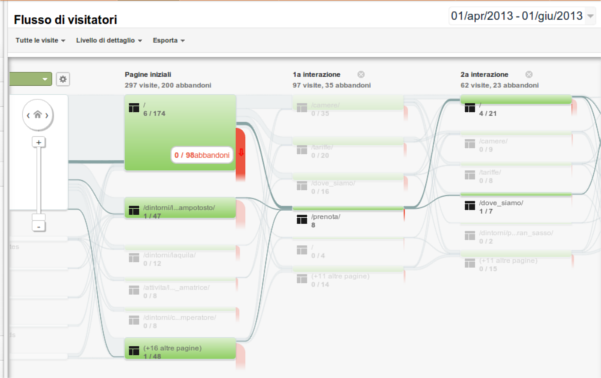
\includegraphics[width=0.80\textwidth,keepaspectratio=true]{../img/googleFlusso}
    \centering
    \caption{Flusso dei visitatori sul sito \url{www.vecchiaposta.it}}%
    \label{fig:googleFlusso}%
  \end{figure}
  \par I due screenshot successivi (fig.\ref{fig:googleAnalyticsPaesi} e fig.\ref{fig:googleAnalyticsBrowser}) mostrano i dati statici che riguardano i paesi di provenenzia
  delle visite e dei browser maggiormanete utilizzati. Sono dati utili per lo sviluppo del nuovo sito, sia per le versioni in lingua straniera sia per verificare
  la completa compatibilità con i vari browser sul mercato.
  \begin{figure}[h!]%
    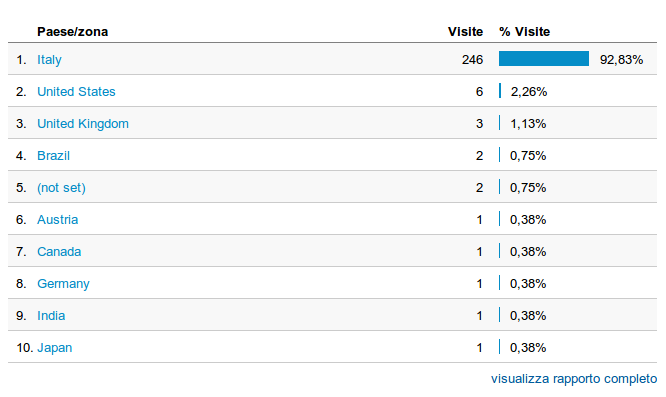
\includegraphics[width=0.80\textwidth,keepaspectratio=true]{../img/googleAnalyticsPaesi}
    \centering
    \caption{Provenienza degli accessi al sito internet}%
    \label{fig:googleAnalyticsPaesi}%
  \end{figure}
  \begin{figure}[h!]%
    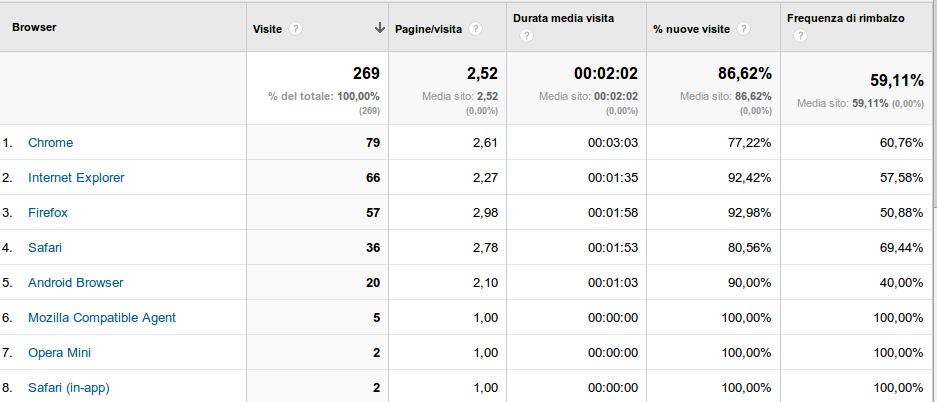
\includegraphics[width=0.80\textwidth,keepaspectratio=true]{../img/googleAnalyticsBrowser}
    \centering
    \caption{Principali browser che accedono al sito}%
    \label{fig:googleAnalyticsBrowser}%
  \end{figure}
  \newpage
  \par In questa ultima immagine, fig.\ref{fig:googleTecnologia}, si porta in evidenza come sia importante rendere il sito maggiormanete usabile da \textit{dispositivi mobile} (tablet, smartphone,
  padfone). 
  \\Infatti dall'analisi dei dati statistici e dalla proiezione dei dati, funzionalità offerta dal servizio di Google Analitycs, si nota come sono in costante 
  aumento le visite tramite l'utilizzo di questi dispositivi.
  \begin{figure}[h!]%
    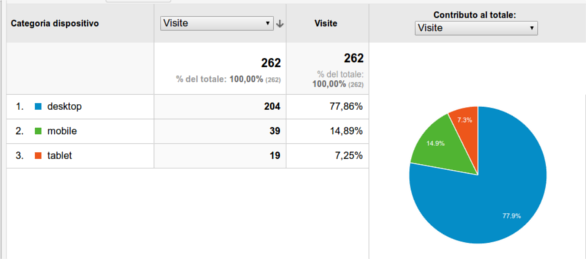
\includegraphics[width=0.80\textwidth,keepaspectratio=true]{../img/googleTecnologia}
    \centering
    \caption{Visite per tipologia di device}%
    \label{fig:googleTecnologia}%
  \end{figure}

  \section{Appendice 2}
  \label{sec:appendice2}
  In questa sezione verranno mostrati i pregi e i difetti dei siti concorrenti analizzati. Anche se la ricerca è stata eseguita su più siti si riportano le considerazioni
  solamente di due siti aziendali locali ed uno non locale che hanno colpito maggiormente il sottoscritto.
  \begin{itemize}
    \item \textbf{B\&B Camaga} (fig. \ref{fig:bebCamaga}): 
      \begin{itemize}
	\item Pro:
	  \begin{itemize}
	    \item Home page leggera: appena 305Kb
	    \item Sito provvisto di una breadcrump\footnote{letteralmente bricola di pane,
	    in internet indica il percorso dell'utente \url{http://it.wikipedia.org/wiki/Breadcrumb}}
	  \end{itemize}
	\item Contro:
	  \begin{itemize}
	    \item Caricamento della home page: anche se leggera ed esegue poche richieste HTTP impiega 14,5 secondi nel caricamento intero della pagina, causa principale è il 
	    caricamento dell'immagine nella home;
	    \item Stile di non gradevole effetto grafico, presenta una side-bar di destra con colori non conformi allo stile, che sembra quasi una pubblicità;
	    \item Nel menu utilizzate etichette forvianti come ``Dove Siamo'' che invece di fornire la posizione del B\&B, cosa che si aspetta, fornisce indicazioni su come 
	    raggiungerlo;
	    \item Header e Menu sono presenti due menu uno laterale in verticale e l'altro appena sotto l'header con il logo/motto del B\&B. Anche in questo caso forse la scelta 
	    grafica non è risultata ottimale, infatti utilizza un font serif per il logo rendendolo quasi illeggibile;
	    \item La cosa più sconvolgente che si riscontra navigando su questo sito è che risulta essere incompleto in molte sue parti
	  \end{itemize}
	  \begin{figure}[h!]%
	    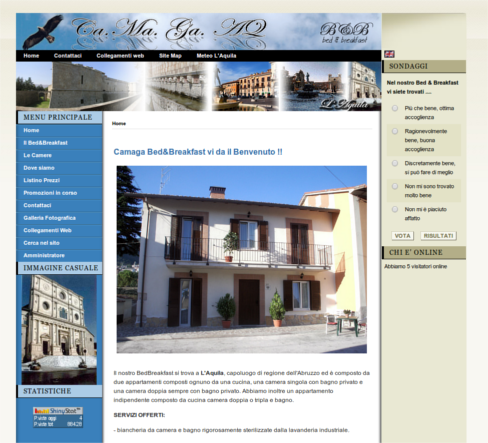
\includegraphics[width=0.95\textwidth,keepaspectratio=true]{../img/bebCamaga}
	    \centering
	    \caption{Screenshot sito: \url{www.camagaaq.com}}%
	    \label{fig:bebCamaga}%
	  \end{figure}
      \item \textbf{La compagnia del viaggiatore} (fig. \ref{fig:bebViaggiatore}):
	\begin{itemize}
	 \item Pro:
	  \begin{itemize}
	   \item Home page curata esteticamente propone una barra di navigazione orizzontale, uno slider e scorciatoie ai servizi principali dell'azienda
	   \item Ogni singola pagina ha al suo interno un proprio slider di immagini
	   \item I caratteri e il tema sono sicuramente scelte  di un esperto del settore
	  \end{itemize}
	 \item Contro:
	  \begin{itemize}
	   \item Breadcrumb non presnte
	   \item Regolazione del font non prevista
	   \item Alcuni contrasti risultano essere privi di effetto, come il verde chiaro su sfondo bianco.
	  \end{itemize}
	\end{itemize}
	\begin{figure}[h!]%
	    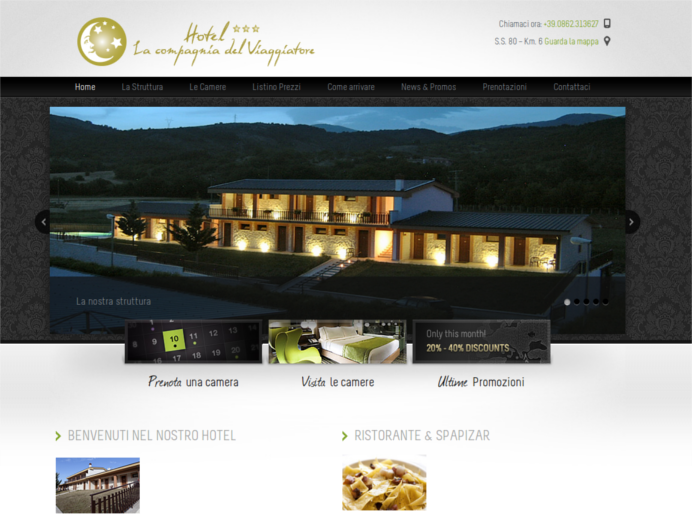
\includegraphics[width=0.95\textwidth,keepaspectratio=true]{../img/bebViaggiatore}
	    \centering
	    \caption{Screenshot sito: \url{http://www.compagniadelviaggiatore.it/}}%
	    \label{fig:bebViaggiatore}%
	  \end{figure}
      \item \textbf{B\&B Il giglio bianco} (fig. \ref{fig:bebGiglio}):
	\begin{itemize}
	 \item Pro:
	  \begin{itemize}
	   \item Home page: contiene tutto quello che serve ad un sito vetrina. Risulta essere gradevole alla vista richiamando inoltre il nome del B\&B avendo il 
	   tema sul bianco
	   \item home page risulta essere leggera con solamente 721Kb caricati in 22 sec, attraverso 85 HTTP Request.
	   \item Grafica sicuramente curata da un professionista del settore mostra scelte ben curate.
	   \item Navigazione presenta due barre una orizzontale ed una verticale che permettono di navigare con facilità il sito.
	   \item il widget booking-online presente in alto a destra nell'header include una funzionalità utilissima per le richieste di prenotazioni
	  \end{itemize}
	 \item Contro:
	  \begin{itemize}
	   \item Le due barre di navigazione non rendono ben comprensibile quale sia la principale e quale la secondaria. A primo impatto il sottoscritto è stato reso in inganno
	   dalla barra verticale pensando fosse una barra di secondo livello per la navigazione nelle sezioni di secondarie
	   \item Non è presente un breadcrump il che rende difficoltosa la navigazione ad un utente non esperto che potrebbe non ricordare il suo percorso di navigazione
	  \end{itemize}
	\end{itemize}
	\begin{figure}[h!]%
	    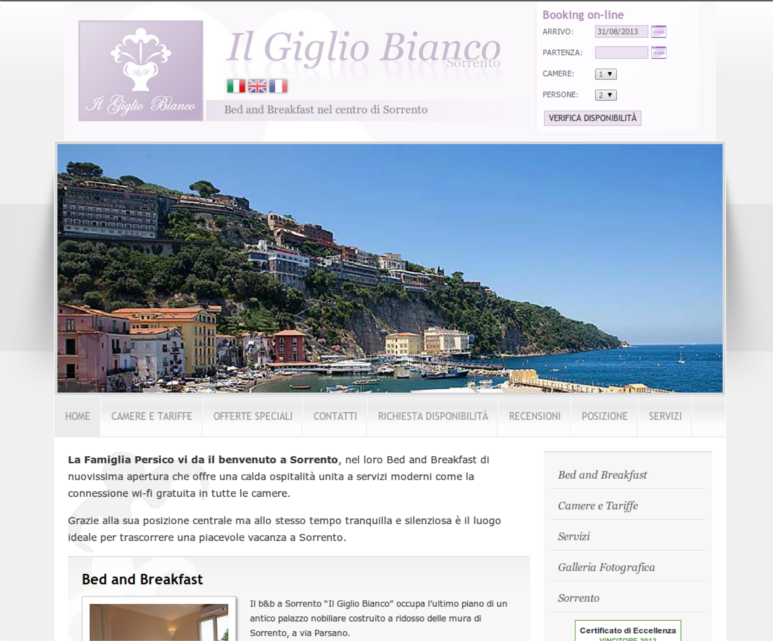
\includegraphics[width=0.80\textwidth,keepaspectratio=true]{../img/bebGiglio}
	    \centering
	    \caption{Screenshot sito: \url{http://www.bbgigliobiancosorrento.it/}}%
	    \label{fig:bebGiglio}%
	\end{figure}
    \end{itemize}
  \end{itemize}
  Riassumendo ciò che si è notato analizzando nel dettaglio i siti proposti e altri non riportati in questo documento, risulta evidente che nella maggioranze dei siti internet
  non è posta l'attenzione sulla navigazione di utente con handicap. Infatti nessuno sito propone un controllo del font lasciando all'utente la sola scelta di utilizzare 
  lo zoom del browser che ovviamente comporta un malfunzionamento dei temi grafici. 
  Anche per quanto riguarda problemi di daltonismi in molti siti sembra esserci poca attenzione, per non parlare della non curanza nell'utilizzo di attributi ALT significativi
  per rendere il sito navigabile tramite browser vocali.

\newpage
\section{Appendice 3}
\label{sec:appendice3}
In questa sezione del documento verranno riportati i principali casi d'uso riscontrati nella prima fase di analisi.
\begin{figure}[h!]%
    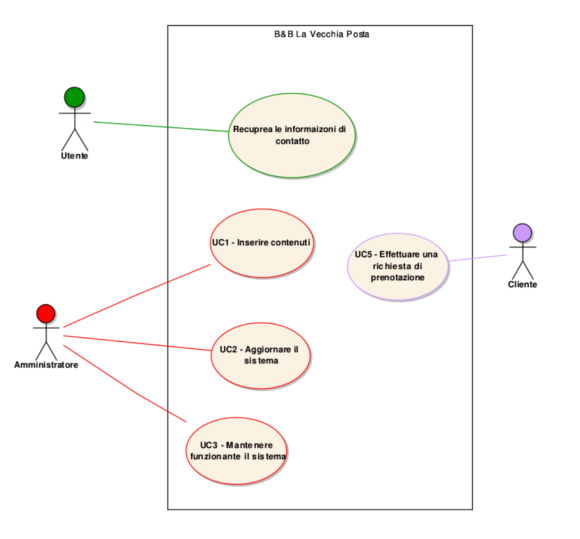
\includegraphics[width=0.85\textwidth,keepaspectratio=true]{../img/useCase}
    \centering
    \caption{Diagramma UML dei casi d'uso}%
    \label{fig:useCase}%
  \end{figure}
  \newpage
Il primo caso d'uso analizzato è quello che vede l'amministratore come utente principale ed è nella fase di dover aggiornare le informazioni presenti nel sito internet.
  
%Sometimes it is a good idea to put domain objects in \texttt{}
%The template and the descriptions are based on the book Applying UML and Patterns: 
%An Introduction to Object-Oriented Analysis and Design and Iterative Development
%(3rd Edition) by Craig Larman.
\begin{usecase}

\addtitle{Caso d'uso:}{UC1 - Inserire Contenuti} 

%Scope: the system under design
\addfield{Scopo:}{Utente}

%Level: "user-goal" or "subfunction"
\addfield{Livello:}{Utente}

%Primary Actor: Calls on the system to deliver its services.
\addfield{Attore primarios:}{Amministratore}

%Stakeholders and Interests: Who cares about this use case and what do they want?

%Preconditions: What must be true on start and worth telling the reader?
% \addfield{Preconditions:}{}
%when multiple
\additemizedfield{Precondizioni:}{
  \item Il sistema ha identificato correttamente l'utente
  \item Il materiale multimediale è pronto per l'inserimento
  
} 

%Postconditions: What must be true on successful completion and worth telling the reader
\addfield{Postcondizioni:}{I contenuti multemediali sono stati aggiornati con successo}
%when multiple
%\additemizedfield{Preconditions:}{}

%Main Success Scenario: A typical, unconditional happy path scenario of success.
\addscenario{Scenario principale di successo:}{
	\item l'amministratore accede al framework
	\item Il sistema mostra all'utente la pagina principale del back-end
	\item l'utente individua la sezione da aggiornare
	\item il sistema mostra correttamente la sezione richiesta
	\item l'utente iserisce/modifica i dati
	\item l'utente salva i dati
	\item il sitema aggiorna i dati 
	\item il sistema avverte l'utente che iul salvataggio è andato a buon fine
	\item l'utente lascia il sistema
}

%Extensions: Alternate scenarios of success or failure.
\addscenario{Estensioni:}{
	\item[4.a] Sezione errata:
		\begin{enumerate}
		\item[1.] il sistema non riesce a mostrare la sezione richiesta
		\item[2.] il sistema invia una email al progettista con il report del bug
		\item[3.] l'utente torna al punto 2
		\end{enumerate}
	\item[6.a] Salvataggio errato:
		\begin{enumerate}
		\item[1.] il sistema non esegue il savataggio
		\item[2.] il sistema mostra l'eventuale errore all'utente
		\item[3.] il sistema invia una mail al progettista con il report del bug
		\item[4.] il sistema mostra all'utente la pagina di provenienza
		\end{enumerate}
}

%Frequency of Occurrence: Influences investigation, testing and timing of implementation.
\addfield{Frequenza:}{ alta nella fase iniziale, bassa nelle fasi successive
}

%Miscellaneous: Such as open issues/questions
%\addfield{Open Issues:}{}

\end{usecase}


Il secondo ed ultimo caso d'uso preso in esame è quello che vede il cliente alle prese con una richiesta di prenotazione.
  
%Sometimes it is a good idea to put domain objects in \texttt{}
%The template and the descriptions are based on the book Applying UML and Patterns: 
%An Introduction to Object-Oriented Analysis and Design and Iterative Development
%(3rd Edition) by Craig Larman.
\begin{usecase}

\addtitle{Caso d'uso:}{UC5 - Effettuare una richiesta di prenotazione} 

%Scope: the system under design
\addfield{Scopo:}{Utente}

%Level: "user-goal" or "subfunction"
\addfield{Livello:}{Utente}

%Primary Actor: Calls on the system to deliver its services.
\addfield{Attore primario:}{Cliente}

%Stakeholders and Interests: Who cares about this use case and what do they want?

%Preconditions: What must be true on start and worth telling the reader?
% \addfield{Preconditions:}{}
%when multiple
\additemizedfield{Precondizioni:}{
  \item Il sito web è navigabile
} 

%Postconditions: What must be true on successful completion and worth telling the reader
\addfield{Postcondizioni:}{La richiesta è avvenuta con successo}
%when multiple
%\additemizedfield{Preconditions:}{}

%Main Success Scenario: A typical, unconditional happy path scenario of success.
\addscenario{Scenario principale di successo:}{
	\item il cliente accede alla pagina web
	\item Il sistema mostra all'utente la pagina home page
	\item l'utente richiede la pagine per le prenotazioni
	\item il sistema mostra correttamente la sezione richiesta
	\item il sistema carica il \textit{form} per l'invio dei dati
	\item l'utente compila i dati del \textit{form} mostrato
	\item l'utente invia i dati
	\item il sistema salva i dati
	\item il sistema invia email all'utente per la corretta ricezione della richiesta
	\item il sistema notifica all'amministratore la richiesta avvenuta
	\item il sistema mostra all'utente la home page
	\item l'utente abbandona il sito
}

%Extensions: Alternate scenarios of success or failure.
\addscenario{Estensioni:}{
	\item[4.a] Pagina richiesta non disponibile:
		\begin{enumerate}
		\item[1.] il sistema non riesce a mostrare la sezione richiesta
		\item[2.] il sistema invia una email al progettista con il report del bug
		\item[3.] il sistema torna al punto 2
		\end{enumerate}
	\item[7.a] Invio errato:
		\begin{enumerate}
		\item[1.] il sistema non esegue l'invio
		\item[2.] il sistema mostra l'eventuale errore all'utente
		\item[3.] il sistema invia una mail al progettista con il report del bug
		\item[4.] il sistema mostra all'utente la pagina di provenienza
		\end{enumerate}
	\item[7.b] Dati inseriti errati:
		\begin{enumerate}
		\item[1.] il sistema non esegue l'invio
		\item[2.] il sistema mostra l'eventuale o gli eventuali dati inseriti errati
		\item[4.] l'utente correggie gli errori
		\item[5.] l'utente esegue il punto 7
		\end{enumerate}
}

%Frequency of Occurrence: Influences investigation, testing and timing of implementation.
\addfield{Frequenza:}{media/alta nelle fasi successive}

%Miscellaneous: Such as open issues/questions
%\addfield{Open Issues:}{}

\end{usecase}


\par I due casi d'uso mostrati precedentemente risultano essere i casi d'uso più comuni e di maggiore rilevanza per quanto riguarda questo documento. Gli altri casi d'uso 
elencati precedentemente risultano essere meno significativi e più banali di quelli dettagliati.
\newpage
\section{Appendice 4}
\label{sec:appendice4}
Gli screenshot riportati sono stati prelevati dal risultato ottenuto dall'analisi effettuata tramite il servizio offerto dal sito \url{http://colorfilter.wickline.org/}. 
\par La mancanza delle immagini è dovuta dal fatto che il servizio non è riuscito ad analizzare i file di immagine presenti nello slider. Si fa inoltre presente che è stato 
analizzato il template del tema e non la versione finale.
\begin{figure}[h!]%
  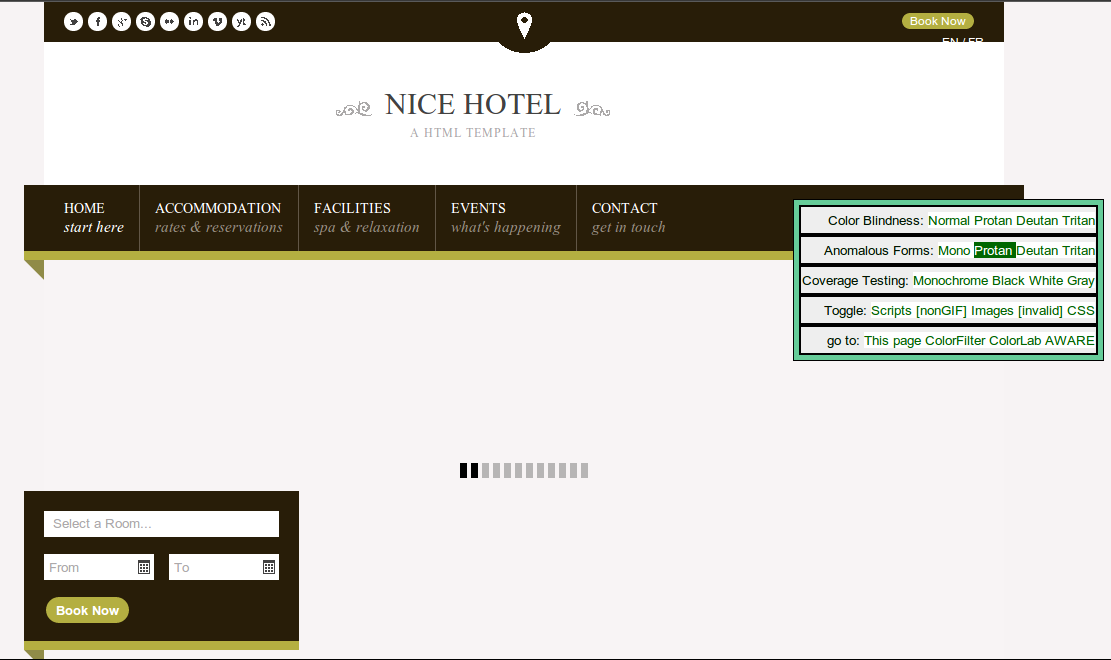
\includegraphics[width=0.95\textwidth,keepaspectratio=true]{../img/daltonismoProtanopia}
  \centering
  \caption{Daltonismo: protanopia}%
  \label{fig:daltonismoProtanopia}%
\end{figure}

\begin{figure}[h!]%
  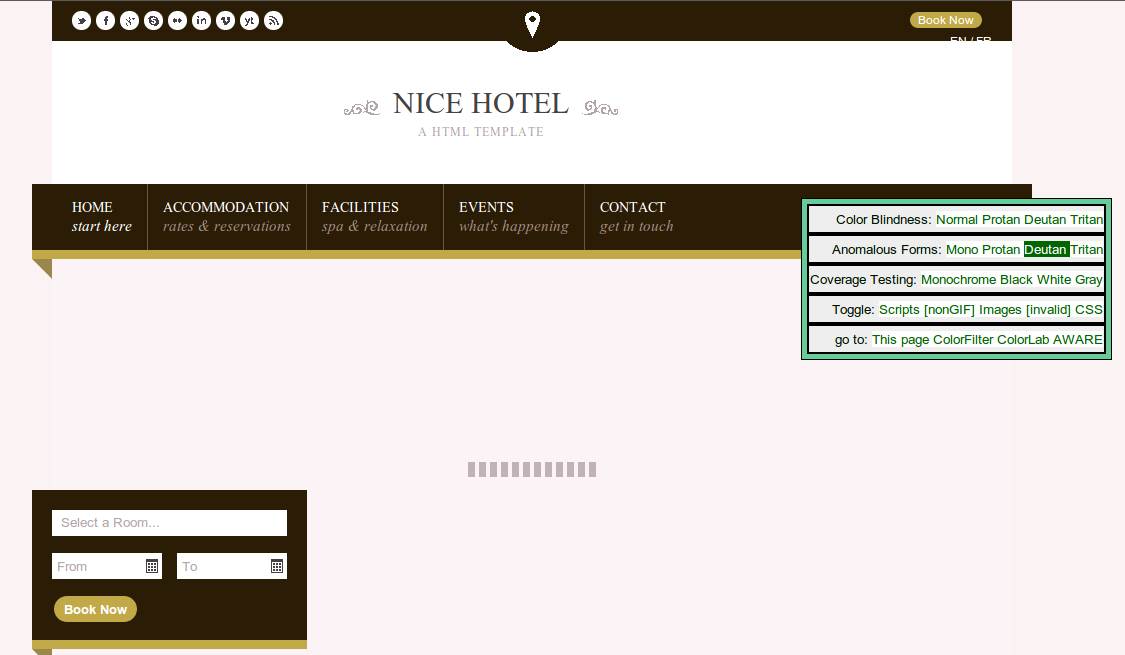
\includegraphics[width=0.95\textwidth,keepaspectratio=true]{../img/daltonismoDeuteranopia}
  \centering
  \caption{Daltonismo: deuteranopia}%
  \label{fig:daltonismoDeuteranopia}%
\end{figure}

\begin{figure}[h!]%
  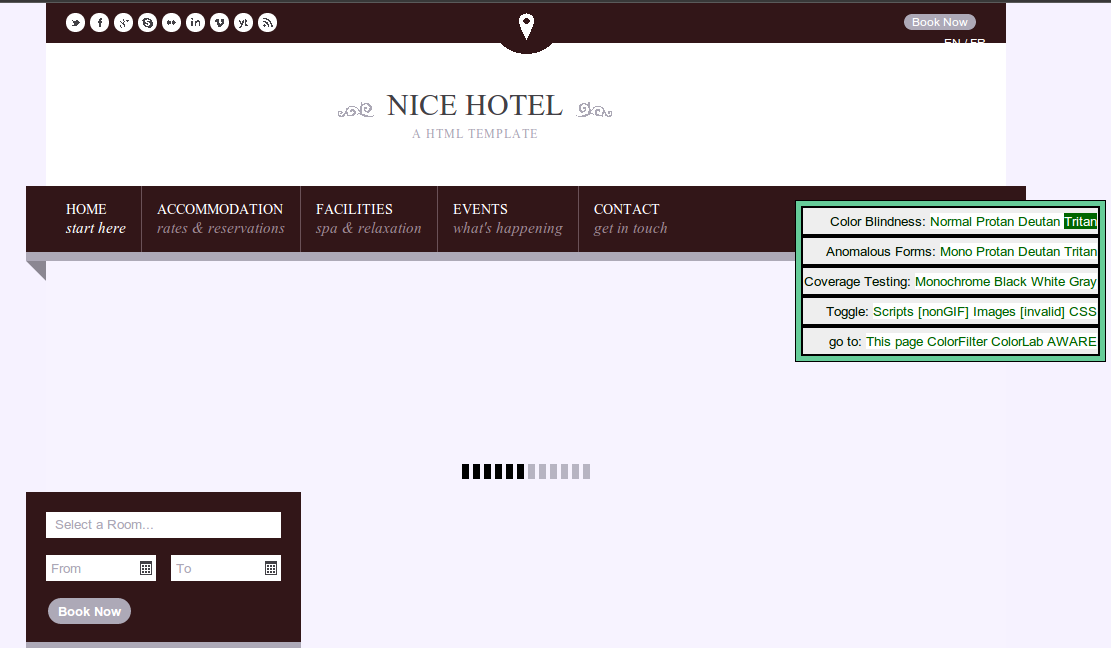
\includegraphics[width=0.95\textwidth,keepaspectratio=true]{../img/daltonismoTritanopia}
  \centering
  \caption{Daltonismo: tritanopia}%
  \label{fig:daltonismoTritanopia}%
\end{figure}
Come si può notare dagli screenshot l'effetto di contrasto è comunque mantenuto non portando gravi anomalie che renderebbero il sito non navigabile dai daltonici. 
\\Sono state analizzate solamente le tre più comuni forme di daltonismo e soprattutto quelle legate maggiormente ai colori scelte nel tema.
\end{document}